\documentclass{article}

\usepackage[utf8]{inputenc}
\usepackage[english]{babel}

\usepackage{amsmath,amsfonts,amssymb}
\usepackage{fullpage}
\usepackage{verbatim}
\usepackage{mathabx}

\usepackage{tikz,pgfplots}

\pgfplotsset{
  width=150mm,height=100mm,
  major grid style={thin,dotted,color=black!50},
  minor grid style={thin,dotted,color=black!50},
  grid,
  every axis/.append style={
    line width=0.5pt,
    tick style={
      line cap=round,
      thin,
      major tick length=4pt,
      minor tick length=2pt,
    },
  },
  legend cell align=left,
  legend pos=north west,
}

%%%%%%%%%%%%%%%%%%%%%%%%%%%%%%%%%%%%%%%%%%%%%%%%%%%%%%%%%%%%%%%%%%%%%%%%%%%%%%%%

\begin{document}

\title{LCE-Queries}
\author{Alexander Herlez}
%\maketitle



% IMPORT-DATA stats statsX

\begin{center}
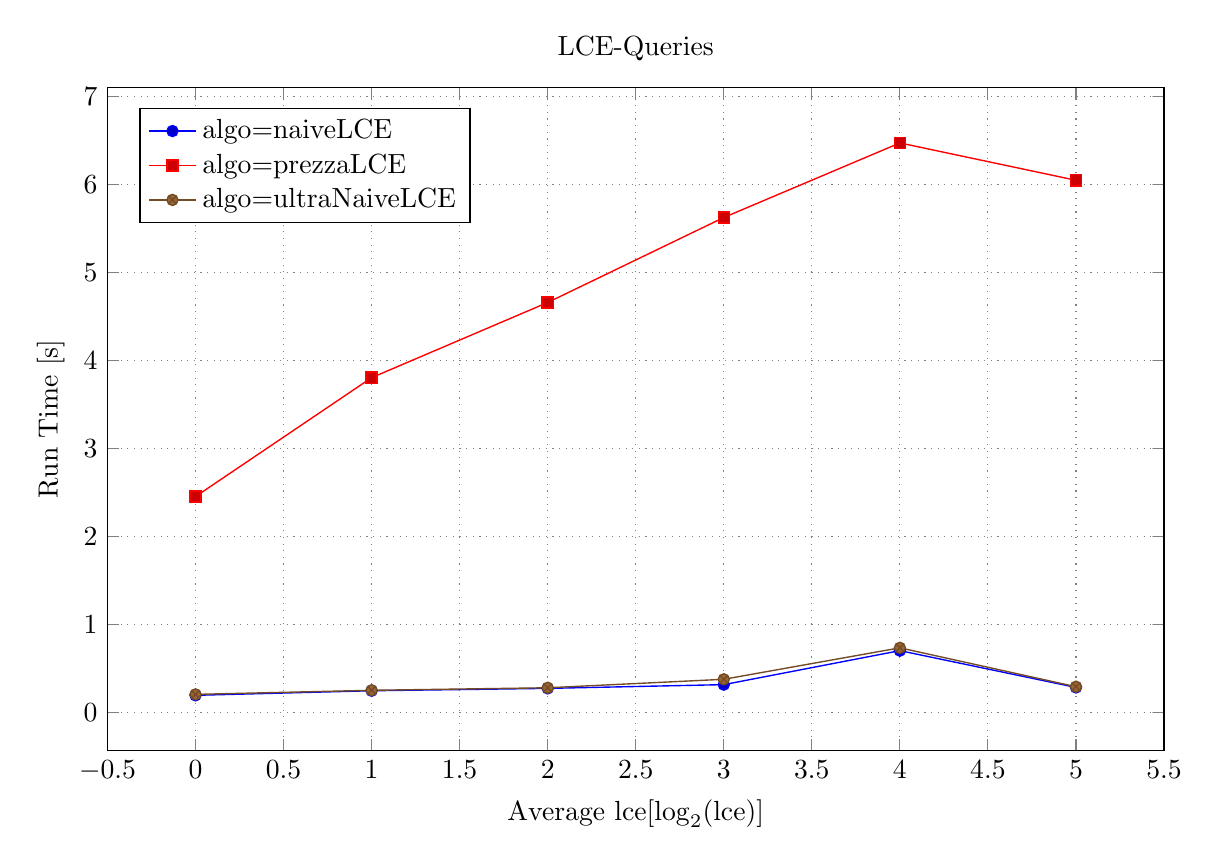
\begin{tikzpicture}
  \begin{axis}[
    title={LCE-Queries},
    xlabel={Average lce[$\log_2$(lce)]},
    ylabel={Run Time [s]},
    ]

    %% MULTIPLOT(algo) SELECT lceLog AS x, time AS y, MULTIPLOT
    %% FROM stats GROUP BY MULTIPLOT,x  ORDER BY MULTIPLOT,x
    \addplot coordinates { (0,0.199853) (1,0.251708) (2,0.278551) (3,0.321091) (4,0.706898) (5,0.289321) };
    \addlegendentry{algo=naiveLCE};
    \addplot coordinates { (0,2.45567) (1,3.80519) (2,4.65863) (3,5.62327) (4,6.46948) (5,6.04566) };
    \addlegendentry{algo=prezzaLCE};
    \addplot coordinates { (0,0.210557) (1,0.256874) (2,0.285435) (3,0.381784) (4,0.738924) (5,0.297512) };
    \addlegendentry{algo=ultraNaiveLCE};

  \end{axis}
\end{tikzpicture}
\end{center}
\end{document}
